\chapter{Implementación, Pruebas y Resultados}
\label{chap:implementacion}

% Colores de los niveles de riesgo (mismos que la plantilla de matriz)
\definecolor{nivMB}{RGB}{198,224,180}
\definecolor{nivB}{RGB}{226,239,218}
\definecolor{nivM}{RGB}{255,235,156}
\definecolor{nivA}{RGB}{248,203,173}
\definecolor{nivMA}{RGB}{255,124,128}

Este capítulo presenta la aplicación de la metodología diseñada en el Capítulo~\ref{chap:metodologia} al caso simulado del proceso de admisión y matrícula de la IES-S. Se describen los productos obtenidos en cada fase, las pruebas realizadas sobre la plantilla y sobre el cumplimiento de los requisitos, y los resultados comparados entre la situación inicial y la situación proyectada tras el tratamiento.

Debe advertirse una condición que atraviesa todo el capítulo: las probabilidades y los impactos registrados son \textbf{estimaciones preliminares del investigador}, cada una acompañada de su justificación, elaboradas para demostrar el funcionamiento de la metodología. Conforme a la Sección~\ref{sec:requerimientos}, estas estimaciones deberán ser revisadas y calibradas por el panel Delphi; los resultados de ese panel y de la validación con expertos se incorporarán cuando concluya su aplicación.

\section{Descripción de la Solución}

La solución implementada es un artefacto metodológico compuesto por cuatro productos:

\begin{enumerate}
  \item \textbf{Documento metodológico}: fases 0 a 4, escalas, tabla de decisión y criterios de aceptación (Sección~\ref{sec:diseno_solucion}).
  \item \textbf{Plantilla reutilizable de matriz de riesgos}: archivo \texttt{matriz/Plantilla\_Matriz\_Riesgos\_LOPDP.xlsx}, con diez hojas, listas desplegables, fórmulas y formato condicional (Anexo~\ref{anx:plantilla_matriz}).
  \item \textbf{Instrumentos de recolección}: lista de verificación normativa, guía de entrevista, cuestionario de madurez, cuestionario Delphi, afirmaciones de calibración, instrumento de validación y consentimiento informado (Anexos~\ref{anx:lista_verificacion} a~\ref{anx:consentimiento}).
  \item \textbf{Matriz aplicada al caso simulado}: archivo \texttt{matriz/Matriz\_Aplicada\_IES-S.xlsx}, con trece escenarios de riesgo del proceso de admisión y matrícula.
\end{enumerate}

La plantilla y la matriz aplicada se generan mediante un programa en JavaScript (\texttt{scripts/build\_matriz.js}) que construye el libro de cálculo, evalúa todas sus fórmulas con un motor de cálculo independiente y reporta los resultados. De este modo, las cifras que se presentan en este capítulo proceden directamente de las fórmulas de la matriz y no de cálculos manuales.

\section{Proceso de Implementación}

\subsection{Fase 0: diagnóstico de madurez}

El cuestionario de madurez (Anexo~\ref{anx:madurez}) y la lista de verificación normativa (Anexo~\ref{anx:lista_verificacion}) se aplicaron sobre la documentación y las prácticas del caso simulado descritas en la Sección~\ref{sec:diagnostico_actual}. La Tabla~\ref{tab:madurez_resultados} resume el nivel de madurez por dominio, calculado como la mediana de sus enunciados.

\begin{table}[htbp]
  \centering
  \caption{Nivel de madurez por dominio en la IES-S (caso simulado).}
  \label{tab:madurez_resultados}
  \footnotesize
  \renewcommand{\arraystretch}{1.2}
  \begin{tabularx}{\textwidth}{|p{3.0cm}|c|c|L|}
    \hline
    \textbf{Dominio} & \textbf{Respuestas} & \textbf{Nivel} & \textbf{Hallazgo principal} \\
    \hline
    Gobernanza & 2, 1, 1 & 1 & Política general sin delegado de protección de datos designado. \\
    \hline
    Inventario y licitud & 1, 2, 1 & 1 & Sin RAT; consentimiento genérico en el formulario de postulación. \\
    \hline
    Gestión de riesgos & 1, 1, 1 & 1 & No se evalúan riesgos para los titulares ni la necesidad de EIPD. \\
    \hline
    Seguridad & 2, 3, 2 & 2 & Respaldos diarios, pero accesos por unidad y sin registro de accesos a datos sensibles. \\
    \hline
    Terceros & 1, 1 & 1 & Contratos con encargados sin cláusulas de protección de datos. \\
    \hline
    Ciclo de vida & 1, 1 & 1 & Conservación indefinida de expedientes. \\
    \hline
    Derechos e incidentes & 2, 1 & 1,5 & Solicitudes atendidas de manera informal; sin procedimiento de notificación. \\
    \hline
    Cultura & 2, 1 & 1,5 & Inducción general sin contenidos de protección de datos. \\
    \hline
    \multicolumn{2}{|l|}{\textbf{Nivel global (mediana)}} & \textbf{1} & \textbf{Inicial} \\
    \hline
  \end{tabularx}
  \raggedright
  \elaboradopor{Ramón Alejandro Manzaba Castro}
  \fuente{Aplicación del Anexo~\ref{anx:madurez} al caso simulado}
\end{table}

La lista de verificación normativa arrojó cero requisitos cumplidos, cinco cumplidos parcialmente (bases de legitimación, información al titular, medidas de seguridad, atención de derechos y capacitación) y diez incumplidos. Entre los incumplimientos destacan la ausencia de una metodología de análisis de riesgos, que la LOPDP tipifica como infracción grave \cite[art.~68]{lopdp2021}, la falta de un procedimiento de notificación de vulneraciones \cite[art.~43]{lopdp2021} y la inexistencia de un dictamen sobre tratamiento a gran escala. El nivel global \textit{inicial} confirma que la institución debe comenzar por las fases de identificación y evaluación antes de abordar controles avanzados.

\subsection{Fase 1: identificación}

\textbf{Establecimiento del contexto.} En el contexto interno, el proceso involucra a cinco unidades y a cuatro encargados del tratamiento, y se concentra en dos ventanas anuales de alta carga operativa. En el contexto externo, el sector educativo presenta una elevada exposición al \textit{ransomware} \cite{sophos2024education} y antecedentes regionales de exfiltración de datos de estudiantes \cite{cnnchile2024usm,semana2023unal}. En el contexto normativo, rigen la LOPDP, su reglamento, la guía de gestión de riesgos de la SPDP y la norma de tratamiento a gran escala \cite{lopdp2021,rlopdp2023,spdp2026guiav2,spdp2026granescala}.

\textbf{Registro de actividades de tratamiento.} La Tabla~\ref{tab:rat} presenta el RAT preliminar del proceso, construido a partir de las entrevistas y de la revisión documental del caso.

\begin{table}[htbp]
  \centering
  \caption{Registro de actividades de tratamiento (RAT) preliminar del proceso de admisión y matrícula.}
  \label{tab:rat}
  \scriptsize
  \renewcommand{\arraystretch}{1.2}
  \begin{tabularx}{\textwidth}{|>{\raggedright\arraybackslash}p{1.8cm}|L|>{\raggedright\arraybackslash}p{2.0cm}|>{\raggedright\arraybackslash}p{2.2cm}|>{\raggedright\arraybackslash}p{2.1cm}|>{\raggedright\arraybackslash}p{1.9cm}|}
    \hline
    \textbf{Subproceso} & \textbf{Finalidad} & \textbf{Base de legitimación (propuesta)} & \textbf{Categorías especiales} & \textbf{Encargados} & \textbf{Conservación actual} \\
    \hline
    SP1 Registro y postulación & Gestionar la postulación del aspirante & Medidas precontractuales; consentimiento para difusión & Datos de adolescentes & CRM de admisiones & Indefinida \\
    \hline
    SP2 Admisión y nivelación & Evaluar y decidir la admisión & Medidas precontractuales & Datos de adolescentes & Suite en la nube & Indefinida \\
    \hline
    SP3 Becas y aranceles & Asignar becas y aranceles diferenciados & Consentimiento explícito; obligación normativa & Discapacidad, salud, condición socioeconómica & Suite en la nube & Indefinida \\
    \hline
    SP4 Pago de matrícula & Cobrar y facturar & Ejecución del contrato; obligación tributaria & Ninguna & Pasarela de pagos & Según normativa tributaria \\
    \hline
    SP5 Legalización & Formalizar la matrícula y crear cuentas & Ejecución del contrato & Ninguna & Suite en la nube; LMS & Mientras dure la relación académica \\
    \hline
    SP6 Reportes y archivo & Reportar a organismos de control y archivar & Obligación legal & Según el reporte & Ninguno & Indefinida (incluye no admitidos) \\
    \hline
  \end{tabularx}
  \raggedright
  \elaboradopor{Ramón Alejandro Manzaba Castro}
  \fuente{Elaboración propia (caso simulado)}
\end{table}

\textbf{Determinación de gran escala.} El proceso trata de forma sistemática datos de adolescentes en un entorno educativo (SP1 y SP2) y datos de salud y discapacidad (SP3). Ambos supuestos constituyen, de forma directa, tratamiento a gran escala según la Resolución SPDP-SPD-2026-0005-R, lo que vuelve obligatorias la evaluación de impacto previa y la designación de un delegado de protección de datos \cite[arts.~12 y 14]{spdp2026granescala}. Esta conclusión, obtenida en la fase de identificación, condiciona el resto de la aplicación: la EIPD no es opcional para la IES-S.

\textbf{Escenarios de riesgo.} A partir del catálogo de amenazas de la plantilla y de las vulnerabilidades halladas en la fase 0, se construyeron trece escenarios de riesgo, cada uno referido a una sola dimensión. La Tabla~\ref{tab:escenarios} los resume; la descripción completa de cada escenario (comunidad de amenaza, vector, vulnerabilidad, control existente y fundamento normativo) consta en la matriz aplicada.

\begin{table}[htbp]
  \centering
  \caption{Escenarios de riesgo identificados en el proceso de admisión y matrícula.}
  \label{tab:escenarios}
  \scriptsize
  \renewcommand{\arraystretch}{1.2}
  \begin{tabularx}{\textwidth}{|c|c|L|>{\raggedright\arraybackslash}p{2.0cm}|>{\raggedright\arraybackslash}p{1.9cm}|}
    \hline
    \textbf{ID} & \textbf{SP} & \textbf{Escenario} & \textbf{Dimensión} & \textbf{Tipo de vulnerabilidad} \\
    \hline
    R-01 & SP3 & Exposición de certificados de discapacidad y fichas socioeconómicas por carpetas compartidas sin restricción & Confidencialidad & Organizacional \\
    \hline
    R-02 & SP1 & Compromiso de cuentas del personal de admisiones por \textit{phishing} y acceso al CRM & Confidencialidad & Técnica \\
    \hline
    R-03 & SP2 & Publicación de listados de admitidos con cédula y puntaje & Licitud & Organizacional \\
    \hline
    R-04 & SP1 & Uso de datos de aspirantes para difusión sin consentimiento específico & Licitud & Jurídica \\
    \hline
    R-05 & SP5 & Consultas indebidas al SGA por privilegios excesivos & Confidencialidad & Organizacional \\
    \hline
    R-06 & SP2 & Alteración de resultados de admisión mediante una cuenta privilegiada comprometida & Integridad & Técnica \\
    \hline
    R-07 & SP4 & Tratamiento por la pasarela de pagos sin garantías contractuales & Confidencialidad & Jurídica \\
    \hline
    R-08 & SP5 & Interrupción del SGA por \textit{ransomware} durante la matrícula & Disponibilidad & Técnica \\
    \hline
    R-09 & SP3 & Exfiltración de expedientes de becas en un ataque de doble extorsión & Confidencialidad & Técnica \\
    \hline
    R-10 & SP6 & Conservación indefinida de expedientes de aspirantes no admitidos & Licitud & Jurídica \\
    \hline
    R-11 & SP3 & Transferencia internacional a la nube sin evaluación de garantías & Licitud & Jurídica \\
    \hline
    R-12 & SP6 & Vulneración no notificada dentro del término legal & Licitud & Organizacional \\
    \hline
    R-13 & SP1 & Indisponibilidad del portal en el cierre de postulaciones & Disponibilidad & Técnica \\
    \hline
  \end{tabularx}
  \raggedright
  \elaboradopor{Ramón Alejandro Manzaba Castro}
  \fuente{Matriz aplicada al caso simulado IES-S}
\end{table}

Los escenarios cubren las cuatro dimensiones y los cuatro tipos de vulnerabilidad previstos por la guía de la SPDP \cite{spdp2026guiav2}: cinco escenarios se originan en vulnerabilidades técnicas, cuatro en jurídicas y cuatro en organizacionales, mientras que la condición de grupo vulnerable de los titulares ---adolescentes y personas con discapacidad--- está presente en ocho de ellos.

\subsection{Fase 2: evaluación}

Para cada escenario se estimó la probabilidad anual y el impacto sobre el titular con la escala de la Sección~\ref{sec:diseno_solucion}, se aplicaron los agravantes y la matriz determinó el impacto ajustado y el nivel inherente mediante la tabla de decisión. La Tabla~\ref{tab:riesgo_inherente} presenta los resultados.

\begin{table}[htbp]
  \centering
  \caption{Riesgo inherente de los escenarios del caso simulado.}
  \label{tab:riesgo_inherente}
  \footnotesize
  \renewcommand{\arraystretch}{1.2}
  \begin{tabular}{|c|c|c|c|c|c|c|}
    \hline
    \textbf{ID} & \textbf{Probabilidad} & \textbf{Impacto (titular)} & \textbf{Agravantes} & \textbf{Impacto ajustado} & \textbf{Nivel inherente} & \textbf{EIPD} \\
    \hline
    R-01 & Media & Alto & 1 & Muy alto & \cellcolor{nivMA}Muy alto & Obligatoria \\
    \hline
    R-02 & Alta & Medio & 1 & Alto & \cellcolor{nivMA}Muy alto & Obligatoria \\
    \hline
    R-03 & Media & Medio & 1 & Alto & \cellcolor{nivA}Alto & Obligatoria \\
    \hline
    R-04 & Muy alta & Bajo & 1 & Medio & \cellcolor{nivA}Alto & Obligatoria \\
    \hline
    R-05 & Alta & Medio & 0 & Medio & \cellcolor{nivA}Alto & Valorar \\
    \hline
    R-06 & Baja & Alto & 0 & Alto & \cellcolor{nivA}Alto & Obligatoria \\
    \hline
    R-07 & Baja & Alto & 0 & Alto & \cellcolor{nivA}Alto & Valorar \\
    \hline
    R-08 & Media & Alto & 1 & Muy alto & \cellcolor{nivMA}Muy alto & Valorar \\
    \hline
    R-09 & Media & Alto & 2 & Muy alto & \cellcolor{nivMA}Muy alto & Obligatoria \\
    \hline
    R-10 & Muy alta & Bajo & 1 & Medio & \cellcolor{nivA}Alto & Valorar \\
    \hline
    R-11 & Media & Medio & 1 & Alto & \cellcolor{nivA}Alto & Obligatoria \\
    \hline
    R-12 & Media & Medio & 0 & Medio & \cellcolor{nivM}Medio & Recomendada \\
    \hline
    R-13 & Media & Bajo & 0 & Bajo & \cellcolor{nivM}Medio & Recomendada \\
    \hline
  \end{tabular}
  \par\vspace{2pt}
  \raggedright
  \elaboradopor{Ramón Alejandro Manzaba Castro}
  \fuente{Matriz aplicada al caso simulado IES-S (estimaciones preliminares)}
\end{table}

Once de los trece escenarios (84,6\,\%) alcanzan un nivel inherente alto o muy alto. Cuatro de ellos son de nivel muy alto: la exposición y la exfiltración de datos de becas (R-01 y R-09), el compromiso de cuentas de admisiones (R-02) y la interrupción del SGA por \textit{ransomware} (R-08). La Figura~\ref{fig:mapas_calor} representa la distribución de los escenarios en el mapa de calor; conforme a la guía de la SPDP, el mapa se usa para comunicar los resultados y no para calibrarlos \cite{spdp2026guiav2}.

\newcommand{\mapabase}{%
  % filas: y=3 Muy alta ... y=0 Muy baja; columnas x=0 Muy bajo ... x=4 Muy alto (escala 1.25 x 0.75)
  \foreach \y/\cs in {3.0/{nivM,nivA,nivA,nivMA,nivMA}, 2.25/{nivB,nivM,nivA,nivMA,nivMA}, 1.5/{nivB,nivM,nivM,nivA,nivMA}, 0.75/{nivMB,nivB,nivM,nivA,nivA}, 0/{nivMB,nivMB,nivB,nivM,nivA}} {
    \foreach \c [count=\i from 0] in \cs { \fill[\c] (\i*1.25,\y) rectangle ++(1.25,0.75); \draw (\i*1.25,\y) rectangle ++(1.25,0.75); }
  }
  \foreach \t [count=\i from 0] in {Muy bajo,Bajo,Medio,Alto,Muy alto} { \node[font=\tiny, rotate=0] at (\i*1.25+0.625,-0.25) {\t}; }
  \foreach \t/\y in {Muy alta/3.0,Alta/2.25,Media/1.5,Baja/0.75,Muy baja/0} { \node[font=\tiny, anchor=east] at (-0.05,\y+0.375) {\t}; }
  \node[font=\scriptsize] at (3.125,-0.6) {Impacto sobre el titular};
}

\begin{figure}[htbp]
  \centering
  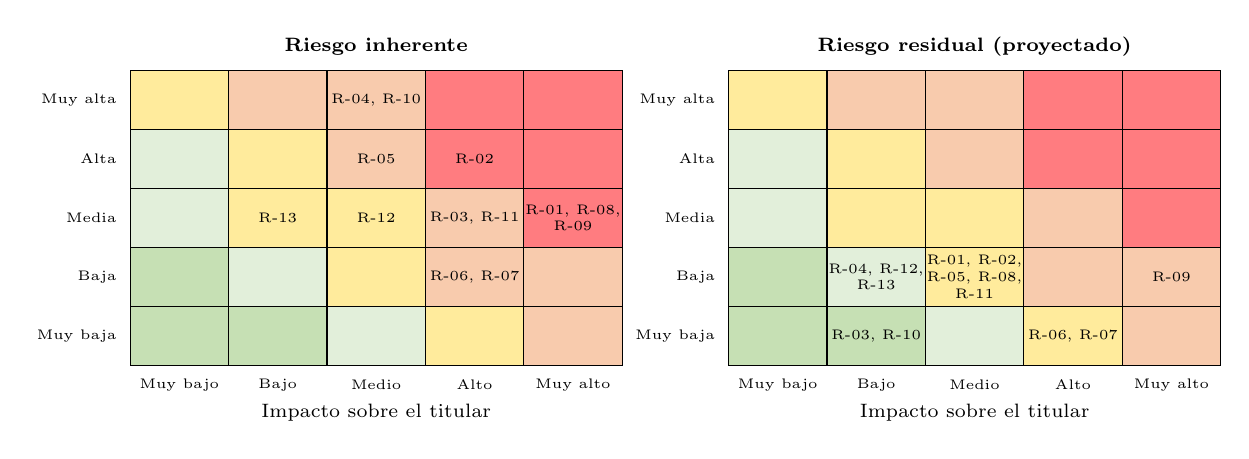
\begin{tikzpicture}
    \begin{scope}
      \mapabase
      \node[font=\scriptsize\bfseries] at (3.125,4.05) {Riesgo inherente};
      \node[font=\tiny] at (2.5+0.625,3.375) {R-04, R-10};
      \node[font=\tiny] at (2.5+0.625,2.625) {R-05};
      \node[font=\tiny] at (3.75+0.625,2.625) {R-02};
      \node[font=\tiny] at (1.25+0.625,1.875) {R-13};
      \node[font=\tiny] at (2.5+0.625,1.875) {R-12};
      \node[font=\tiny] at (3.75+0.625,1.875) {R-03, R-11};
      \node[font=\tiny, align=center] at (5.0+0.625,1.875) {R-01, R-08,\\R-09};
      \node[font=\tiny] at (3.75+0.625,1.125) {R-06, R-07};
    \end{scope}
    \begin{scope}[xshift=7.6cm]
      \mapabase
      \node[font=\scriptsize\bfseries] at (3.125,4.05) {Riesgo residual (proyectado)};
      \node[font=\tiny, align=center] at (1.25+0.625,1.125) {R-04, R-12,\\R-13};
      \node[font=\tiny, align=center] at (2.5+0.625,1.125) {R-01, R-02,\\R-05, R-08,\\R-11};
      \node[font=\tiny] at (5.0+0.625,1.125) {R-09};
      \node[font=\tiny] at (1.25+0.625,0.375) {R-03, R-10};
      \node[font=\tiny] at (3.75+0.625,0.375) {R-06, R-07};
    \end{scope}
  \end{tikzpicture}
  \caption{Mapas de calor del riesgo inherente y residual del caso simulado.}
  \label{fig:mapas_calor}
  \raggedright
  \elaboradopor{Ramón Alejandro Manzaba Castro}
  \fuente{Matriz aplicada al caso simulado IES-S}
\end{figure}

\textbf{Dictamen de evaluación de impacto.} Además de ser obligatoria por la calificación de gran escala, la EIPD se justifica por el resultado de la evaluación: siete escenarios de nivel alto o muy alto involucran categorías especiales de datos o titulares de grupos vulnerables. El subproceso SP3 (becas y aranceles diferenciados) concentra los escenarios más graves (R-01, R-09 y R-11), por lo que se priorizó para la EIPD. La Tabla~\ref{tab:eipd_sp3} resume sus elementos principales.

\begin{table}[htbp]
  \centering
  \caption{Síntesis de la EIPD del subproceso de becas y aranceles diferenciados (SP3).}
  \label{tab:eipd_sp3}
  \footnotesize
  \renewcommand{\arraystretch}{1.25}
  \begin{tabularx}{\textwidth}{|p{3.3cm}|L|}
    \hline
    \textbf{Elemento} & \textbf{Contenido} \\
    \hline
    Descripción del tratamiento & Recolección, verificación y conservación de fichas socioeconómicas y certificados de discapacidad de aproximadamente 1\,200 postulantes por año, para asignar becas y aranceles diferenciados. \\
    \hline
    Necesidad y proporcionalidad & La condición socioeconómica y la discapacidad son necesarias para asignar el beneficio; no lo es conservar copia del certificado una vez verificado ni mantener los expedientes de postulantes sin beca. \\
    \hline
    Riesgos para los titulares & Discriminación y exclusión de beneficios por exposición (R-01, R-09); pérdida de control por transferencias sin garantías (R-11). \\
    \hline
    Medidas previstas & Minimización (registrar solo la verificación), clasificación y control de acceso, autenticación multifactor, cifrado en reposo, prevención de fuga, evaluación de la transferencia y cláusulas con el proveedor. \\
    \hline
    Riesgo residual & Medio en R-01 y R-11; alto en R-09, porque el impacto sobre el titular se mantiene muy alto aunque disminuya la probabilidad. \\
    \hline
    Conclusión & El tratamiento puede continuar si se implementan las medidas previstas; el riesgo residual de R-09 requiere las observaciones del delegado de protección de datos y del área jurídica y la aprobación de la máxima autoridad, y debe considerarse la eliminación de los certificados tras su verificación para reducir el impacto. \\
    \hline
  \end{tabularx}
  \raggedright
  \elaboradopor{Ramón Alejandro Manzaba Castro}
  \fuente{Elaboración propia con base en \cite{lopdp2021,spdp2026guiav2,iso29134_2023}}
\end{table}

\subsection{Fase 3: mitigación}

Para cada escenario se eligió una opción de tratamiento, se propusieron controles con referencia a ISO/IEC 27002:2022 \cite{iso27002_2022} y se estimó el riesgo residual bajo el supuesto de que los controles se implementen. La Tabla~\ref{tab:plan_tratamiento} presenta el plan de tratamiento. Conforme a las exclusiones del proyecto, la implementación de estas medidas corresponde a la institución.

\begin{table}[htbp]
  \centering
  \caption{Plan de tratamiento y riesgo residual proyectado.}
  \label{tab:plan_tratamiento}
  \scriptsize
  \renewcommand{\arraystretch}{1.2}
  \begin{tabularx}{\textwidth}{|c|>{\raggedright\arraybackslash}p{1.25cm}|L|>{\raggedright\arraybackslash}p{1.1cm}|c|c|c|}
    \hline
    \textbf{ID} & \textbf{Opción} & \textbf{Controles principales (ISO/IEC 27002:2022)} & \textbf{Plazo} & \textbf{Prob. res.} & \textbf{Imp. res.} & \textbf{Nivel residual} \\
    \hline
    R-01 & Mitigar & 5.12 clasificación; 5.15 control de acceso; 8.5 MFA; 8.12 prevención de fuga; minimización & 3 meses & Baja & Medio & \cellcolor{nivM}Medio \\
    \hline
    R-02 & Mitigar & 8.5 MFA; 6.3 concienciación; 5.18 revisión de accesos; minimización del formulario & 2 meses & Baja & Medio & \cellcolor{nivM}Medio \\
    \hline
    R-03 & Evitar & 8.11 enmascaramiento: publicar solo el código de postulante & Próximo periodo & Muy baja & Bajo & \cellcolor{nivMB}Muy bajo \\
    \hline
    R-04 & Mitigar & 5.34 consentimiento por finalidad y aviso de privacidad; 5.31 requisitos legales & 1 mes & Baja & Bajo & \cellcolor{nivB}Bajo \\
    \hline
    R-05 & Mitigar & 5.15 acceso por función; 5.18 revisión por periodo; 8.15 registro de accesos & 4 meses & Baja & Medio & \cellcolor{nivM}Medio \\
    \hline
    R-06 & Mitigar & 8.2 cuentas privilegiadas nominativas; 8.5 MFA; 8.15 registro de cambios & 3 meses & Muy baja & Alto & \cellcolor{nivM}Medio \\
    \hline
    R-07 & Transferir & 5.19 y 5.20 cláusulas de protección de datos y notificación de incidentes & 6 meses & Muy baja & Alto & \cellcolor{nivM}Medio \\
    \hline
    R-08 & Mitigar & 8.13 respaldos aislados y probados; 8.8 vulnerabilidades; 8.7 malware; 5.24 y 5.26 incidentes & 4 meses & Baja & Medio & \cellcolor{nivM}Medio \\
    \hline
    R-09 & Mitigar & 8.24 cifrado en reposo; 8.12 prevención de fuga; 8.16 monitoreo; 8.10 eliminación & 6 meses & Baja & Muy alto & \cellcolor{nivA}Alto \\
    \hline
    R-10 & Mitigar & 8.10 eliminación periódica según tabla de conservación; 5.9 inventario & 6 meses & Muy baja & Bajo & \cellcolor{nivMB}Muy bajo \\
    \hline
    R-11 & Mitigar & 5.19 y 5.20 acuerdos con el proveedor; 5.31 evaluación de la transferencia & 4 meses & Baja & Medio & \cellcolor{nivM}Medio \\
    \hline
    R-12 & Mitigar & 5.24 y 5.26 procedimiento de respuesta y notificación; simulacro anual & 2 meses & Baja & Bajo & \cellcolor{nivB}Bajo \\
    \hline
    R-13 & Mitigar & 8.6 gestión de la capacidad; acuerdo de nivel de servicio & Próximo periodo & Baja & Bajo & \cellcolor{nivB}Bajo \\
    \hline
  \end{tabularx}
  \raggedright
  \elaboradopor{Ramón Alejandro Manzaba Castro}
  \fuente{Matriz aplicada al caso simulado IES-S}
\end{table}

Tras el tratamiento proyectado, solo el escenario R-09 conserva un nivel alto. Este resultado ilustra la regla de la tabla de decisión para los escenarios de alto impacto: aunque los controles reducen la probabilidad de exfiltración a baja, el daño potencial sobre titulares con discapacidad sigue siendo muy alto, por lo que el riesgo no desciende de nivel alto y no puede aceptarse sin las observaciones del delegado de protección de datos y del área jurídica y la aprobación de la máxima autoridad. La única forma de reducirlo es actuar sobre el impacto, por ejemplo eliminando los certificados una vez verificados. Los escenarios R-06 y R-07 muestran el caso contrario: con impacto alto y probabilidad muy baja, el riesgo residual queda en nivel medio y debe tratarse dentro del plan anual.

\subsection{Fase 4: monitoreo}

La Tabla~\ref{tab:indicadores} define los indicadores de monitoreo asociados a los escenarios de mayor nivel, junto con su meta y su frecuencia de revisión.

\begin{table}[htbp]
  \centering
  \caption{Indicadores de monitoreo del riesgo.}
  \label{tab:indicadores}
  \footnotesize
  \renewcommand{\arraystretch}{1.2}
  \begin{tabularx}{\textwidth}{|c|L|c|>{\raggedright\arraybackslash}p{2.4cm}|}
    \hline
    \textbf{Escenarios} & \textbf{Indicador} & \textbf{Meta} & \textbf{Frecuencia} \\
    \hline
    R-01 & Enlaces públicos detectados en carpetas restringidas & 0 & Mensual \\
    \hline
    R-02, R-06 & Porcentaje de cuentas con autenticación multifactor & 100\,\% & Mensual \\
    \hline
    R-02 & Tasa de clics en simulaciones de \textit{phishing} & $<5$\,\% & Por periodo de admisión \\
    \hline
    R-05 & Porcentaje de perfiles revisados al cierre de cada periodo & 100\,\% & Por periodo académico \\
    \hline
    R-07, R-11 & Porcentaje de encargados con cláusulas de protección de datos & 100\,\% & Semestral \\
    \hline
    R-08 & Tiempo de restauración en la prueba de respaldo & $<24$~h & Trimestral \\
    \hline
    R-09 & Porcentaje de repositorios sensibles cifrados & 100\,\% & Trimestral \\
    \hline
    R-10 & Expedientes vencidos sin eliminar & 0 & Semestral \\
    \hline
    R-12 & Vulneraciones notificadas dentro del término legal & 100\,\% & Por incidente; simulacro anual \\
    \hline
  \end{tabularx}
  \raggedright
  \elaboradopor{Ramón Alejandro Manzaba Castro}
  \fuente{Matriz aplicada al caso simulado IES-S}
\end{table}

El procedimiento de respuesta a vulneraciones, que atiende el escenario R-12, se estructura en cinco pasos: (1) detección y registro del incidente; (2) contención y evaluación inicial, en las primeras 24 horas, para determinar si hay datos personales afectados; (3) valoración del riesgo para los titulares con las escalas de la metodología; (4) notificación a la SPDP dentro del término de cinco días previsto en el artículo~43 de la LOPDP \cite[art.~43]{lopdp2021} y comunicación a los titulares cuando corresponda, y (5) análisis posterior, actualización de la matriz y retroalimentación a la fase de identificación. La matriz se revisa, además, al cierre de cada periodo de admisión y ante cualquier cambio relevante de sistemas, proveedores o normativa.

\section{Pruebas y Validación}

\subsection{Verificación de la plantilla de matriz}

Las fórmulas de la plantilla se evaluaron con un motor de cálculo independiente (HyperFormula) en el momento de generar cada archivo. La plantilla y la matriz aplicada contienen 1\,057 fórmulas cada una y ninguna produjo errores; las cuatro celdas que emplean la función \texttt{QUARTILE}, que ese motor no implementa, se verificaron con un cálculo equivalente en JavaScript. Además, se diseñaron seis casos de prueba para comprobar las reglas de decisión de la metodología. La Tabla~\ref{tab:pruebas} muestra que todos produjeron el resultado esperado.

\begin{table}[htbp]
  \centering
  \caption{Casos de prueba de las reglas de decisión de la plantilla.}
  \label{tab:pruebas}
  \scriptsize
  \renewcommand{\arraystretch}{1.2}
  \begin{tabularx}{\textwidth}{|c|L|>{\raggedright\arraybackslash}p{3.2cm}|>{\raggedright\arraybackslash}p{3.2cm}|c|}
    \hline
    \textbf{Caso} & \textbf{Regla verificada} & \textbf{Entrada} & \textbf{Resultado obtenido} & \textbf{Estado} \\
    \hline
    T-01 & Impacto muy alto con probabilidad muy baja no desciende de nivel alto & P = Muy baja; I = Muy alto & Nivel inherente: Alto & Correcto \\
    \hline
    T-02 & Probabilidad muy alta con impacto muy bajo no se trata como riesgo alto & P = Muy alta; I = Muy bajo & Nivel inherente: Medio & Correcto \\
    \hline
    T-03 & Los agravantes no superan el nivel muy alto & I = Alto; 3 agravantes & Impacto ajustado: Muy alto & Correcto \\
    \hline
    T-04 & Una fila incompleta no genera nivel ni errores & Sin probabilidad & Celdas de resultado vacías & Correcto \\
    \hline
    T-05 & Riesgo residual alto sin categoría especial no es aceptable & PR = Media; IR = Alto & Nivel residual: Alto; ``No aceptable: tratamiento prioritario'' & Correcto \\
    \hline
    T-06 & Impacto residual muy alto exige aprobación reforzada & PR = Muy baja; IR = Muy alto & Nivel residual: Alto; requiere DPD/jurídico y máxima autoridad & Correcto \\
    \hline
  \end{tabularx}
  \raggedright
  \elaboradopor{Ramón Alejandro Manzaba Castro}
  \fuente{Ejecución de \texttt{scripts/build\_matriz.js} con los casos de prueba}
\end{table}

\subsection{Verificación del cumplimiento de los requisitos}

La Tabla~\ref{tab:verificacion_rf} contrasta los requisitos funcionales de la Sección~\ref{sec:requerimientos} con la evidencia generada en la aplicación al caso simulado.

\begin{table}[htbp]
  \centering
  \caption{Verificación de los requisitos funcionales en el caso simulado.}
  \label{tab:verificacion_rf}
  \scriptsize
  \renewcommand{\arraystretch}{1.2}
  \begin{tabularx}{\textwidth}{|c|L|c|}
    \hline
    \textbf{Requisito} & \textbf{Evidencia en la aplicación} & \textbf{Estado} \\
    \hline
    RF01 & Diagnóstico de madurez por dominio (Tabla~\ref{tab:madurez_resultados}) & Cumple \\
    \hline
    RF02 & RAT preliminar de seis subprocesos (Tabla~\ref{tab:rat}) & Cumple \\
    \hline
    RF03 & Vulnerabilidades jurídicas, organizacionales, técnicas y de grupos vulnerables (Tabla~\ref{tab:escenarios}) & Cumple \\
    \hline
    RF04 & Trece escenarios con comunidad de amenaza, vector, vulnerabilidad e impacto en el titular y en el responsable (matriz aplicada) & Cumple \\
    \hline
    RF05 & Probabilidad anual con justificación en cada escenario & Cumple (pendiente calibración Delphi) \\
    \hline
    RF06 & Escenarios separados por confidencialidad, integridad, disponibilidad y licitud & Cumple \\
    \hline
    RF07 & Agravantes aplicados y justificados en ocho escenarios & Cumple \\
    \hline
    RF08 & Nivel inherente y residual por tabla de decisión; regla de alto impacto verificada (T-01, T-06, R-09) & Cumple \\
    \hline
    RF09 & Determinación de gran escala y dictamen de EIPD (Tabla~\ref{tab:eipd_sp3}) & Cumple \\
    \hline
    RF10 & Plan de tratamiento con opción, controles, responsable y plazo (Tabla~\ref{tab:plan_tratamiento}) & Cumple \\
    \hline
    RF11 & Indicadores y procedimiento de respuesta a vulneraciones (Tabla~\ref{tab:indicadores}) & Cumple \\
    \hline
  \end{tabularx}
  \raggedright
  \elaboradopor{Ramón Alejandro Manzaba Castro}
  \fuente{Elaboración propia}
\end{table}

\subsection{Validación con expertos}

La validación de la metodología se realiza con el panel de expertos descrito en el Capítulo~\ref{chap:metodologia}, en dos momentos: (a) la calibración de los expertos con las afirmaciones del Anexo~\ref{anx:calibracion} y la estimación Delphi de la probabilidad y el impacto de los trece escenarios (Anexo~\ref{anx:delphi}), cuyos resultados reemplazarán las estimaciones preliminares, y (b) la valoración de la metodología con el instrumento del Anexo~\ref{anx:validacion}, en el que un criterio se considera validado cuando la mediana del panel es igual o mayor que 4.

\textit{[PENDIENTE: resultados de la calibración (puntaje de Brier por experto), de las rondas Delphi (mediana, RIC y consenso por escenario) y de la validación por juicio de expertos (mediana por criterio V01--V12 y observaciones). Se incorporarán al concluir la aplicación de los instrumentos con el panel.]}

\section{Resultados}

La Tabla~\ref{tab:antes_despues} compara la situación inicial del caso simulado con la situación proyectada tras la aplicación de la metodología y la implementación del plan de tratamiento.

\begin{table}[htbp]
  \centering
  \caption{Comparación de la situación inicial y la proyectada en el caso simulado.}
  \label{tab:antes_despues}
  \footnotesize
  \renewcommand{\arraystretch}{1.2}
  \begin{tabular}{|l|c|c|}
    \hline
    \textbf{Indicador} & \textbf{Inicial} & \textbf{Proyectado} \\
    \hline
    Escenarios de nivel muy alto & 4 & 0 \\
    \hline
    Escenarios de nivel alto & 7 & 1 \\
    \hline
    Escenarios de nivel medio & 2 & 7 \\
    \hline
    Escenarios de nivel bajo o muy bajo & 0 & 5 \\
    \hline
    Escenarios de nivel alto o muy alto (\%) & 84,6\,\% & 7,7\,\% \\
    \hline
    Escenarios con riesgo aceptable sin condiciones & 0 & 5 \\
    \hline
    Actividades de tratamiento inventariadas (RAT) & 0 & 6 \\
    \hline
    Dictamen de gran escala y EIPD & No & Sí \\
    \hline
  \end{tabular}
  \par\vspace{2pt}
  \raggedright
  \elaboradopor{Ramón Alejandro Manzaba Castro}
  \fuente{Matriz aplicada al caso simulado IES-S}
\end{table}

La reducción de los escenarios de nivel alto o muy alto se calcula con la Ecuación~\ref{eq:reduccion}:

\begin{equation}
\label{eq:reduccion}
\text{Reducción (\%)} = \frac{N_{\text{inicial}} - N_{\text{proyectado}}}{N_{\text{inicial}}} \times 100 = \frac{11 - 1}{11} \times 100 = \text{90,9 \%}
\end{equation}
\addeqtolist{Reducción porcentual de escenarios de nivel alto o muy alto}

Estos resultados deben interpretarse con dos cautelas. Primero, el riesgo residual es \textit{proyectado}: supone que los controles propuestos se implementan con eficacia, lo que excede el alcance del proyecto. Segundo, las estimaciones son preliminares y pueden variar tras la calibración con el panel Delphi. Aun así, la aplicación demuestra que la metodología permite pasar de una situación sin inventario, sin evaluación de riesgos y sin dictamen de EIPD a un conjunto trazable de escenarios priorizados, con controles, responsables, plazos e indicadores, que es precisamente la evidencia de responsabilidad proactiva que exigen los artículos 37, 40 y 42 de la LOPDP \cite{lopdp2021}.

\section{Cronograma y Presupuesto}

\subsection{Cronograma}

El proyecto se ejecuta en 24 semanas, distribuidas en las cinco fases de la investigación. La Figura~\ref{fig:cronograma} presenta el cronograma.

\begin{figure}[htbp]
  \centering
  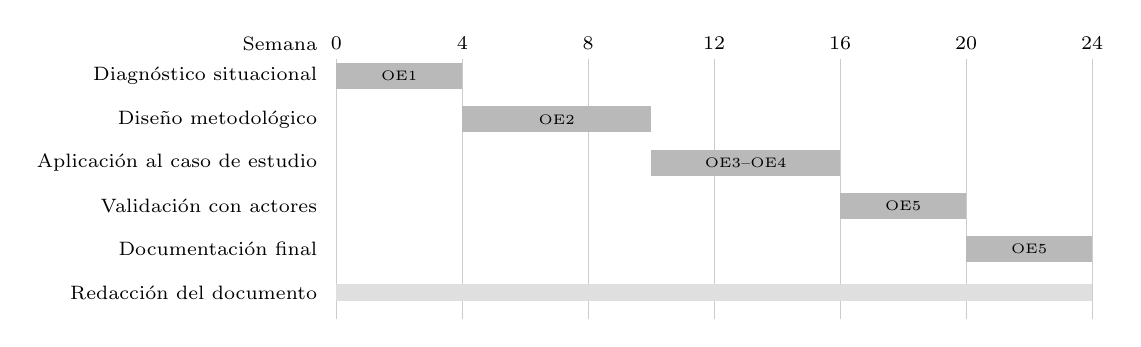
\begin{tikzpicture}[x=0.4cm, y=0.55cm, font=\scriptsize]
    % rejilla de semanas
    \foreach \s in {0,4,...,24} { \draw[gray!40] (\s,0.4) -- (\s,-5.6); \node at (\s,0.75) {\s}; }
    \node[anchor=east] at (-0.3,0.75) {Semana};
    \foreach \y/\nombre/\ini/\fin/\oe in {
        0/Diagnóstico situacional/0/4/OE1,
        -1/Diseño metodológico/4/10/OE2,
        -2/Aplicación al caso de estudio/10/16/OE3--OE4,
        -3/Validación con actores/16/20/OE5,
        -4/Documentación final/20/24/OE5} {
      \node[anchor=east] at (-0.3,\y) {\nombre};
      \fill[gray!55] (\ini,\y-0.3) rectangle (\fin,\y+0.3);
      \node[font=\tiny] at ({(\ini+\fin)/2},\y) {\oe};
    }
    \node[anchor=east] at (-0.3,-5) {Redacción del documento};
    \fill[gray!25] (0,-5.2) rectangle (24,-4.8);
  \end{tikzpicture}
  \caption{Cronograma del proyecto.}
  \label{fig:cronograma}
  \raggedright
  \elaboradopor{Ramón Alejandro Manzaba Castro}
  \fuente{Elaboración propia}
\end{figure}

\subsection{Presupuesto}

La Tabla~\ref{tab:presupuesto} presenta el presupuesto referencial del proyecto. El componente principal es el tiempo del investigador, valorado como costo de oportunidad; el software empleado es libre o se dispone mediante licencias institucionales. El costo de las normas ISO/IEC depende de si se accede a ellas mediante la biblioteca institucional o se adquieren; por ello no se incluye en el subtotal.

\begin{table}[htbp]
  \centering
  \caption{Presupuesto referencial del proyecto (USD).}
  \label{tab:presupuesto}
  \footnotesize
  \renewcommand{\arraystretch}{1.2}
  \begin{tabularx}{\textwidth}{|L|c|r|r|}
    \hline
    \textbf{Rubro} & \textbf{Cantidad} & \textbf{Costo unitario} & \textbf{Total} \\
    \hline
    Tiempo del investigador (costo de oportunidad) & 960 h & 5,00 & 4\,800,00 \\
    \hline
    Equipo de cómputo propio (depreciación de 6 meses) & 1 & 100,00 & 100,00 \\
    \hline
    Software: LaTeX (MiKTeX), Node.js, hoja de cálculo & -- & 0,00 & 0,00 \\
    \hline
    Normas ISO/IEC 27005, 27002 y 29134 & 3 & [VERIFICAR] & [VERIFICAR] \\
    \hline
    Internet y energía & 6 meses & 30,00 & 180,00 \\
    \hline
    Impresión y empastado & 1 & 60,00 & 60,00 \\
    \hline
    \textbf{Subtotal} & & & \textbf{5\,140,00} \\
    \hline
    Imprevistos (5\,\%) & & & 257,00 \\
    \hline
    \textbf{Total referencial} & & & \textbf{5\,397,00} \\
    \hline
  \end{tabularx}
  \raggedright
  \elaboradopor{Ramón Alejandro Manzaba Castro}
  \fuente{Elaboración propia (valores referenciales)}
\end{table}
